\documentclass[12pt,a4paper]{article}

% Packages
\usepackage[utf8]{inputenc}
\usepackage[T1]{fontenc}
\usepackage{lmodern}
\usepackage[margin=2.5cm]{geometry}
\usepackage{hyperref}
\usepackage{graphicx}
\usepackage{listings}
\usepackage{xcolor}
\usepackage{booktabs}
\usepackage{longtable}
\usepackage{array}
\usepackage{enumitem}
\usepackage{titlesec}
\usepackage{fancyhdr}
\usepackage{amsmath}
\usepackage{microtype}
\usepackage{parskip}
\usepackage{tikz}
\usepackage{float}
\usepackage{amsmath}
\usepackage{hyperref}



\usetikzlibrary{
	positioning,
	calc,
	arrows.meta,
	shadows,
	fadings,
	shapes.geometric
}

\title{Lab User Survival Guide}
\author{Lab Team}
\date{\today}

\begin{document}
	
	\begin{titlepage}
		\noindent
		\rule{\textwidth}{0.8pt}
		
		\vspace{0.5cm}
		\thispagestyle{empty}
		\centering
		
		\vspace*{1.5cm}
		
		{\Huge\bfseries LABORATORY USER'S\par}
		\vspace{0.4cm}
		{\Huge\bfseries SURVIVAL GUIDE\par}
		
		\vspace{2cm}
		
		
\includegraphics[width=5cm]{NTNU hovedlogo - farger - hoyde.pdf}
		
		\vspace{2cm}
\noindent
\rule{0.25\textwidth}{0.8pt}
\hfill
\begin{minipage}{0.35\textwidth}
	\centering
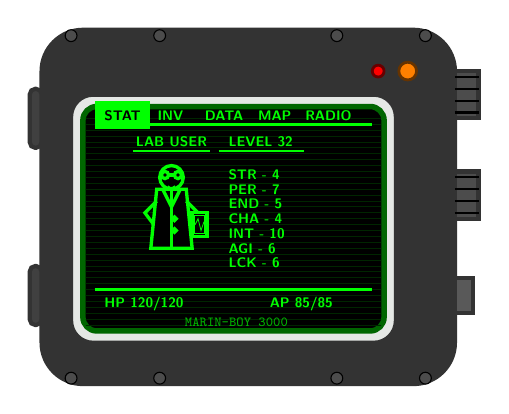
\begin{tikzpicture}[
    scale=0.75,
every node/.style={scale=1},
	c_casing/.style={
		color=darkgray!80!black,
		fill=gray!40!black,
		line width=1.5pt
	},
	c_screen/.style={
		color=green!40!black,
		fill=black,
		line width=2pt
	},
	c_text/.style={
		green,
		font=\sffamily\bfseries\tiny
	}
	]
			
			% =========================================================================
			% 1. PIP-BOY OUTER CASING
			% =========================================================================
			
			\draw[c_casing, rounded corners=15pt]
			(-3.5,-3) rectangle (3.5,3);
			
			\draw[c_casing, rounded corners=10pt]
			(-3.3,-2.8) rectangle (3.3,2.8);
			
			% Screws
			\foreach \x in {-3,-1.5,1.5,3}
			{
				\draw[fill=gray!60!black,draw=black]
				(\x,2.9) circle (0.1cm);
				
				\draw[fill=gray!60!black,draw=black]
				(\x,-2.9) circle (0.1cm);
			}
			
			% Right-side controls
			\draw[c_casing,fill=gray!60!black]
			(3.5,1.5) rectangle (3.9,2.3);
			
			\draw[c_casing,fill=gray!60!black]
			(3.5,-0.2) rectangle (3.9,0.6);
			
			\draw[c_casing,fill=gray!70!black]
			(3.5,-1.8) rectangle (3.8,-1.2);
			
			\foreach \y in {1.6,1.8,2.0,2.2,-0.1,0.1,0.3,0.5}
			{
				\draw[black,line width=0.8pt]
				(3.5,\y)--(3.9,\y);
			}
			
			% Left hinges
			\draw[c_casing,fill=gray!50!black,rounded corners=2pt]
			(-3.7,1.0) rectangle (-3.5,2.0);
			
			\draw[c_casing,fill=gray!50!black,rounded corners=2pt]
			(-3.7,-2.0) rectangle (-3.5,-1.0);
			
			% Lights
			\draw[orange!40!black,fill=orange,line width=1pt]
			(2.7,2.3) circle (0.15cm);
			
			\draw[red!40!black,fill=red,line width=1pt]
			(2.2,2.3) circle (0.10cm);
			
			% =========================================================================
			% SCREEN
			% =========================================================================
			
			\draw[c_casing,fill=black!90!green!10,rounded corners=8pt]
			(-3.0,-2.3) rectangle (2.5,1.9);
			
			\draw[c_screen,rounded corners=5pt]
			(-2.8,-2.1) rectangle (2.3,1.7);
			
			% Scanlines
			\begin{scope}
				\clip (-2.75,-2.05) rectangle (2.25,1.65);
				
				\foreach \y in {-2.0,-1.9,...,1.6}
				{
					\draw[green!15!black,line width=0.3pt]
					(-2.8,\y)--(2.3,\y);
				}
			\end{scope}
			
			% =========================================================================
			% TOP MENU
			% =========================================================================
			
			\draw[green,line width=1pt]
			(-2.6,1.4)--(2.1,1.4);
			
			\node[c_text,anchor=west,fill=green,text=black]
			at (-2.6,1.55) {STAT};
			
			\node[c_text,anchor=west] at (-1.7,1.55) {INV};
			\node[c_text,anchor=west] at (-0.9,1.55) {DATA};
			\node[c_text,anchor=west] at (0.0,1.55) {MAP};
			\node[c_text,anchor=west] at (0.8,1.55) {RADIO};
			
% =========================================================================
% SCIENTIST LABEL
% =========================================================================

% Name heading
\node[
green,
font=\sffamily\bfseries\tiny
]
at (-1.30,1.10) {LAB USER};

% Underline under name
\draw[green,line width=0.5pt]
(-1.95,0.95)--(-0.65,0.95);

% Level heading (same font size)
\node[
green,
font=\sffamily\bfseries\tiny,
anchor=west
]
at (-0.50,1.10) {LEVEL 32};

% Underline under level
\draw[green,line width=0.5pt]
(-0.50,0.95)--(0.95,0.95);

% =========================================================================
% SCIENTIST
% =========================================================================

\begin{scope}[shift={(-1.30,-0.10)},green,line width=1.2pt]
	
	% Head
	\draw[fill=black] (0,0.6) circle (0.2cm);
	
	% Glasses
	\draw (-0.11,0.64) circle (0.06cm);
	\draw (0.11,0.64) circle (0.06cm);
	\draw (-0.05,0.64)--(0.05,0.64);
	
	% Smile
	\draw (-0.07,0.44) arc (-140:-40:0.09);
	
	% Coat
	\draw[fill=black]
	(-0.25,0.4)--(0.25,0.4)--(0.35,-0.6)--(-0.35,-0.6)--cycle;
	
	\draw (0,0.4)--(0,-0.6);
	\draw (-0.15,0.4)--(0,0.1)--(0.15,0.4);
	
	\draw[fill=green] (0.05,-0.1) circle (0.03cm);
	\draw[fill=green] (0.05,-0.3) circle (0.03cm);
	
	% Device
	\draw (0.25,0.2)--(0.45,0.0)--(0.38,-0.15);
	
	\draw[fill=black]
	(0.35,-0.4) rectangle (0.6,0.0);
	
	\draw[line width=0.5pt]
	(0.38,-0.35) rectangle (0.57,-0.05);
	
	\draw[line width=0.3pt]
	(0.4,-0.2)--(0.45,-0.1)--(0.5,-0.3)--(0.55,-0.15);
	
	% Arm
	\draw (-0.25,0.2)--(-0.45,0.0)--(-0.3,-0.2);
	
\end{scope}

% =========================================================================
% STATS
% =========================================================================

\begin{scope}[shift={(-0.70,0.00)}]
	


	
	% Stat list begins BELOW the level heading
	\node[c_text,anchor=west] at (0.2,0.55) {STR - 4};
	\node[c_text,anchor=west] at (0.2,0.30) {PER - 7};
	\node[c_text,anchor=west] at (0.2,0.05) {END - 5};
	\node[c_text,anchor=west] at (0.2,-0.20) {CHA - 4};
	\node[c_text,anchor=west] at (0.2,-0.45) {INT - 10};
	\node[c_text,anchor=west] at (0.2,-0.70) {AGI - 6};
	\node[c_text,anchor=west] at (0.2,-0.95) {LCK - 6};
	
\end{scope}
			
			% Bottom line
			\draw[green,line width=1pt]
			(-2.6,-1.4)--(2.1,-1.4);
			
			% HP
			\node[c_text,anchor=west]
			at (-2.6,-1.65) {HP 120/120};
			

			
			% AP
			\node[c_text,anchor=west]
			at (0.2,-1.65) {AP 85/85};
			

			
			% Footer
			\node[
			green!70!black,
			font=\tiny\ttfamily,
			anchor=center
			]
			at (-0.2,-1.95)
			{MARIN-BOY 3000};
			
		\end{tikzpicture}
	\end{minipage}
	\hfill
	\rule{0.25\textwidth}{0.8pt}
		\vfill

		

		

		
	\end{titlepage}
	\clearpage
	\thispagestyle{empty}
	
	\vspace*{\fill}
	
	\begin{center}
		{\fontsize{50}{60}\selectfont\bfseries DON'T PANIC}
		
		\vspace{1cm}
		
	{\Large
		If the model is upside down (in reality or only in the data),\\
		the coordinate frames are backwards,\\
		the data stream has vanished,\\
		or the experiment is producing revolutionary and/or unexplained results,
	}
		
		\vspace{1cm}
		
		{\LARGE\bfseries
			take a deep breath and keep reading.
		}
		
		\vspace{2cm}
		
		\rule{0.6\textwidth}{0.5pt}
		
		\vspace{0.5cm}
		
\begin{minipage}{0.75\textwidth}
	\centering
	\itshape
	Most problems begin with somebody pressing the wrong button.\\
	Most solutions begin with somebody reading the manual.\\[0.5em]
	You are likely one, or both, of these beings.
\end{minipage}	
		
	\end{center}
	
	\vspace*{\fill}
	
	\clearpage
	\tableofcontents
	\listoffigures
	\listoftables
	\section{Introduction}
	Welcome, Lab User.
	This guide serves as a practical reference for the systems and equipment used throughout the laboratories. In addition to describing the purpose and operation of each system, it contains troubleshooting procedures for the most common issues that may be encountered during laboratory work.
	
	The objective of this guide is to enable users to diagnose and resolve simple problems independently, particularly outside normal working hours when immediate assistance may not be available.
	
	The guide is organized by system type. Each section introduces a particular system, while laboratory-specific configurations and procedures are presented in dedicated subsections where necessary
	\section{Motion Capture System}
	\label{sec:mocap}
	% ============================================================
	
	\subsection{Startup Procedure}
	
	This section describes the standard startup procedure for most users of the motion capture system. If your project requires a different setup or configuration, contact the laboratory engineers before proceeding.
	
	\subsubsection{Quick Startup Checklist}
	
	% Short checklist for experienced users
	
	\subsubsection{Qualisys Track Manager Startup}
	
	
	Open QTM (Qualisys Track Manager). When the \textit{Manage Projects} window appears, select \texttt{Qualisys\_Default\textlangle NAME OF LAB\textrangle}. Press \texttt{Ctrl + N} to open a new measurement window.
	
	Verify that the number of connected cameras displayed in the status bar matches the number of cameras currently in use.
	
	In the toolbar on the left, select \textit{3D View}. This displays the laboratory coordinate system, which is defined as follows:
	

\begin{itemize}
	\item The $x$-axis points toward the wavemaker.
	\item The $z$-axis points downward.
	\item The $y$-axis completes the right-handed coordinate system and points from the gangway toward the opposite side of the basin.
	\item The origin is placed as close to the center of the basin as possible. At the time of writing, its exact position may vary between calibrations.
	\item The coordinate system orientation and origin location are established during calibration, which is normally performed by laboratory personnel. If your project requires the exact origin position or a different coordinate system orientation, contact the laboratory engineers before starting.
\end{itemize}

Press \texttt{Ctrl + D} to open the \textit{Data Info} window. By default, this window displays marker data and coordinates.

Right-click anywhere in the window and select \textit{Display 6DOF Data}. The window will then display the position and orientation of all defined rigid bodies:

\[
x,\; y,\; z,\; \text{roll},\; \text{pitch},\; \text{yaw}
\]

The displayed data also includes the \textit{residual}\footnote{
	The rigid body residual is the average error, measured in millimeters, between the observed marker positions and the corresponding points in the rigid body definition.
	\url{https://docs.qualisys.com/qtm/content/qtm_user_interface/qtm_windows/6dof_data_information.htm?Highlight=residual}
}.

Note that QTM displays position coordinates ($x$, $y$, and $z$) in millimeters and orientation angles (roll, pitch, and yaw) in degrees.

You may now place the vessel in the basin. If the vessel is tracked correctly in QTM and the residual remains sufficiently low, the system is ready for use. Keep in mind that residuals may increase in regions with limited camera coverage or areas that were not fully included during calibration. The calibrated volume can be visualized by pressing \texttt{Alt + 7}.

If the vessel is not detected correctly or the residual remains high ($>1$ mm), continue to Section~\ref{sec:rigidbody}.

\subsubsection{Rigid Body Setup and Verification}
\label{sec:rigidbody}

If the model has not already been defined, or if you are using a different vessel, the corresponding rigid body definitions must be loaded or created.

Open the \textit{Project Options} window by clicking the gear icon in the upper-left toolbar. Navigate to \textit{Processing} $\rightarrow$ \textit{6DOF Tracking}.



If the model has not previously been defined, or if you need to create a new rigid body definition, follow the procedure described below.

% Add rigid body creation procedure here.

Place the model in the basin. Only one model should be present during rigid body acquisition. Remove other models from the basin or cover their markers to prevent false detections. It is important that it is in view of as many cameras as possible(clicking \textit{2D} on the left takes you back to \textit{camera view} which is helpful here). The initial position($x,y,z$) doesn't matter, but make sure that the vessel heading is aligned with the desired heading corresponding to $0^\circ$ yaw, if it is important for your experiment also make sure that the vessel is balanced, the reason for this is that when you acquire a rigid body QTM sets ($roll, pitch,yaw)=(0,0,0)$. 

Go to \textit{6DOF settings} window in the \textit{Project Options}, press \textit{Acquire Body} button. Verify that the body has been detected and then click \textit{Apply} and then \textit{OK}. Close the measurement window by pressing the lower of the two crosses in the top right corner. Open a new measurement window and repeat the steps up until you see the rigid body coordinates in 6-DOF. 

For the first time user it might seem that everything is in order. One should be able to see the rigid body defined by the markers as well as its coordinates in 6DOF, but QTM uses the centroid of the markers defining a rigid body as the body frame origin which does not correspond to the model geometric center. To remedy this all  models should have a reference marker. Lab engineers should have provided you with its position relative to the model geometric center and the model waterline 

Find the marker in QTM corresponding to the reference marker on the model. Select the marker and note its label. The label will typically have the format \texttt{Body1-x} or a similar name if the rigid body has previously been renamed. Return to \emph{6DOF Tracking} settings, select the rigid body and click \emph{Translate}. 

\begin{center}
	\emph{So that point [marker label] in the body has local coordinates (in mm):}
\end{center}
Enter the values for the model in question and press \emph{OK}, press apply and verify that the body has moved the origin of the system. 


% Verifying streaming to downstream systems

\subsection{Common Failure Modes and Symptoms}
\subsubsection{Incorrect Body Frame Origin}
\textbf{Symptoms}
\begin{itemize}
	\item The model appears offset from its expected position in the global reference frame.
	\item Reported position does not correspond to the physical location of the model.
	\item Position appears shifted relative to other tracked objects.
\end{itemize}

\textbf{Possible Causes}
\begin{itemize}
	\item The rigid body origin in QTM was defined at the centroid of the marker constellation instead of being translated to the desired model reference point.
	\item The reference marker coordinates were entered incorrectly.
	\item The rigid body definition was recreated or modified without applying the required translation.
\end{itemize}

\textbf{Recommended Actions}
\begin{itemize}
	\item Verify the location of the rigid body origin in QTM.
	\item Use the model reference marker whose position relative to the model's geometric center and waterline is known.
	\item In the 6DOF tracking settings, use the \emph{Translate} function and assign the reference marker its known coordinates $(x,y,z)$ in the model reference frame.
	\item This translates the rigid body coordinate system such that the body frame origin coincides with the desired model reference point.
\end{itemize}
\subsubsection{Low Marker Count}

\textbf{Symptoms}
\begin{itemize}
	\item Fewer markers than expected are visible in QTM.
	\item 6DOF tracking is unstable or unavailable.
\end{itemize}

\textbf{Possible Causes}
\begin{itemize}
	\item Cameras are blocked by personnel or equipment.
	\item Markers are covered by water spray or reflections.
	\item One or more markers have detached from the model.
	\item Poor camera exposure settings.
\end{itemize}

\textbf{Recommended Actions}
\begin{itemize}
	\item Verify that all markers are attached and clearly visible.
	\item Remove any obstructions from the camera field of view.
	\item Check the camera images for poor contrast or excessive reflections.
\end{itemize}

\subsubsection{High Residuals}

\textbf{Symptoms}
\begin{itemize}
	\item Residual values exceed the normal operating range ($\approx 1$ mm).
	\item Position and orientation estimates appear noisy.
	\item Sudden jumps occur in the measured pose.
\end{itemize}

\textbf{Possible Causes}
\begin{itemize}
	\item Markers have shifted due to a collision or other physical impact.
	\item Incorrect rigid body definition.
	\item Marker misidentification.
	\item Inadequate camera coverage.
	\item Calibration inaccuracies.
\end{itemize}

\textbf{Recommended Actions}
\begin{itemize}
	\item Verify that the correct rigid body definition is loaded.
	\item Check that all markers are correctly identified.
	\item Move the model to an area with better camera coverage.
	\item Remove the rigid body from 6DOF tracking and reacquire it.
\end{itemize}

\subsubsection{Tracking Dropouts}

\textbf{Symptoms}
\begin{itemize}
	\item The model disappears from the 6DOF data stream.
	\item Position data contains gaps.
	\item The body repeatedly loses and regains tracking.
\end{itemize}

\textbf{Possible Causes}
\begin{itemize}
	\item Too few markers are visible to the camera system.
	\item Temporary obstruction by personnel or equipment.
\end{itemize}

\textbf{Recommended Actions}
\begin{itemize}
	\item Check marker visibility in the 3D view.
	\item Ensure that at least three markers remain visible to the system.
	\item Remove obstacles from the capture volume.
\end{itemize}

\subsubsection{Camera System Mismatch}

\textbf{Symptoms}
\begin{itemize}
	\item The number of connected cameras differs from the expected configuration.
	\item One or more camera views are missing.
	\item QTM displays camera connection warnings.
\end{itemize}

\textbf{Possible Causes}
\begin{itemize}
	\item A camera is powered off.
	\item Network or synchronization cables are disconnected.
	\item An incorrect QTM project was loaded.
	\item A camera may be experiencing network or synchronization issues. In this case, contact laboratory personnel.
\end{itemize}

\textbf{Recommended Actions}
\begin{itemize}
	\item Confirm that the correct project is loaded.
	\item Verify that all cameras are powered and connected.
	\item Contact laboratory personnel if a camera remains unavailable.
\end{itemize}

\subsection{Screenshots and Examples}
\begin{figure}[H]
	\centering
	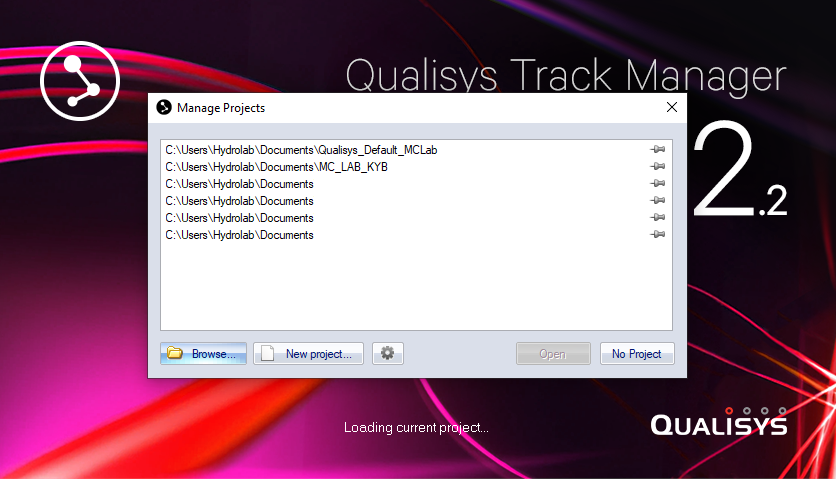
\includegraphics[width=0.5\textwidth]{QTM/1StartupWindow}
	\caption{The first window that appears when starting QTM. Here you will select your project or create a new one}
	\label{fig:manageprojects}
\end{figure}

\begin{figure}[H]
	\centering
	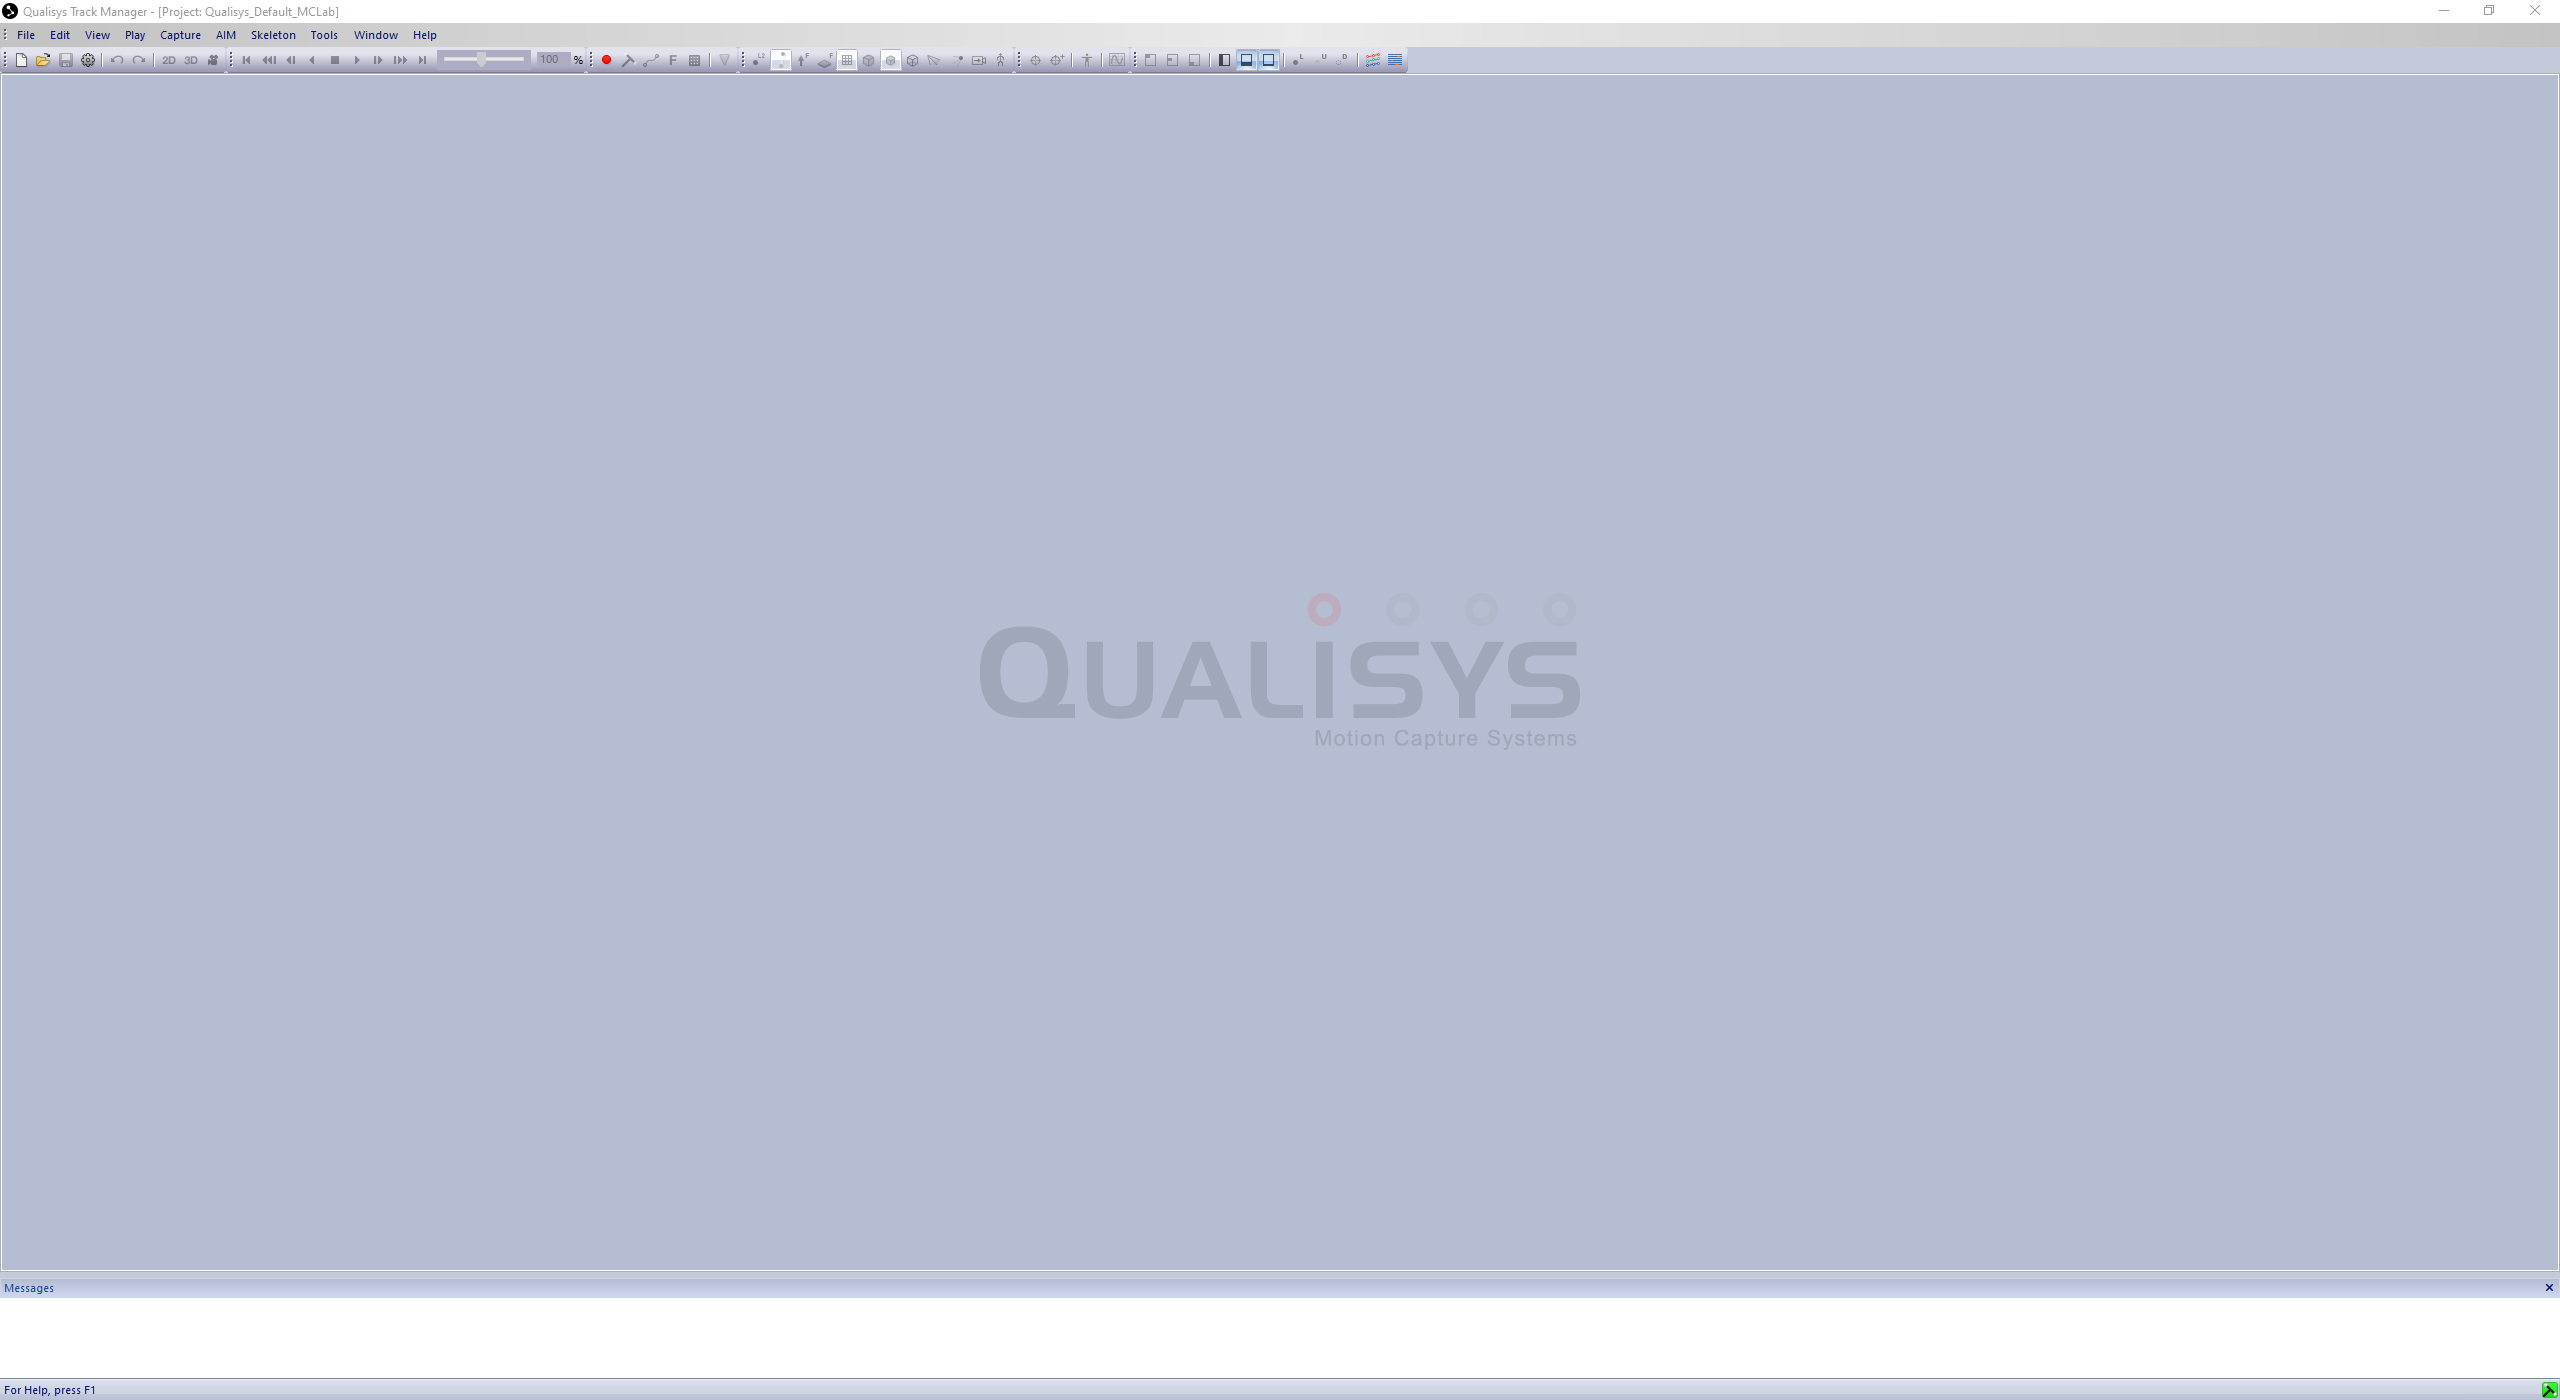
\includegraphics[width=0.5\textwidth]{QTM/2NewMeasurment}
	\caption{Start a new measurement window by clicking the white sheet in the top left or pressing \texttt{CTRL + N}. You must also repeat this if the qualisys system crashes.}
	\label{fig:MeasurmentWindow}
\end{figure}

\begin{figure}[H]
	\centering
	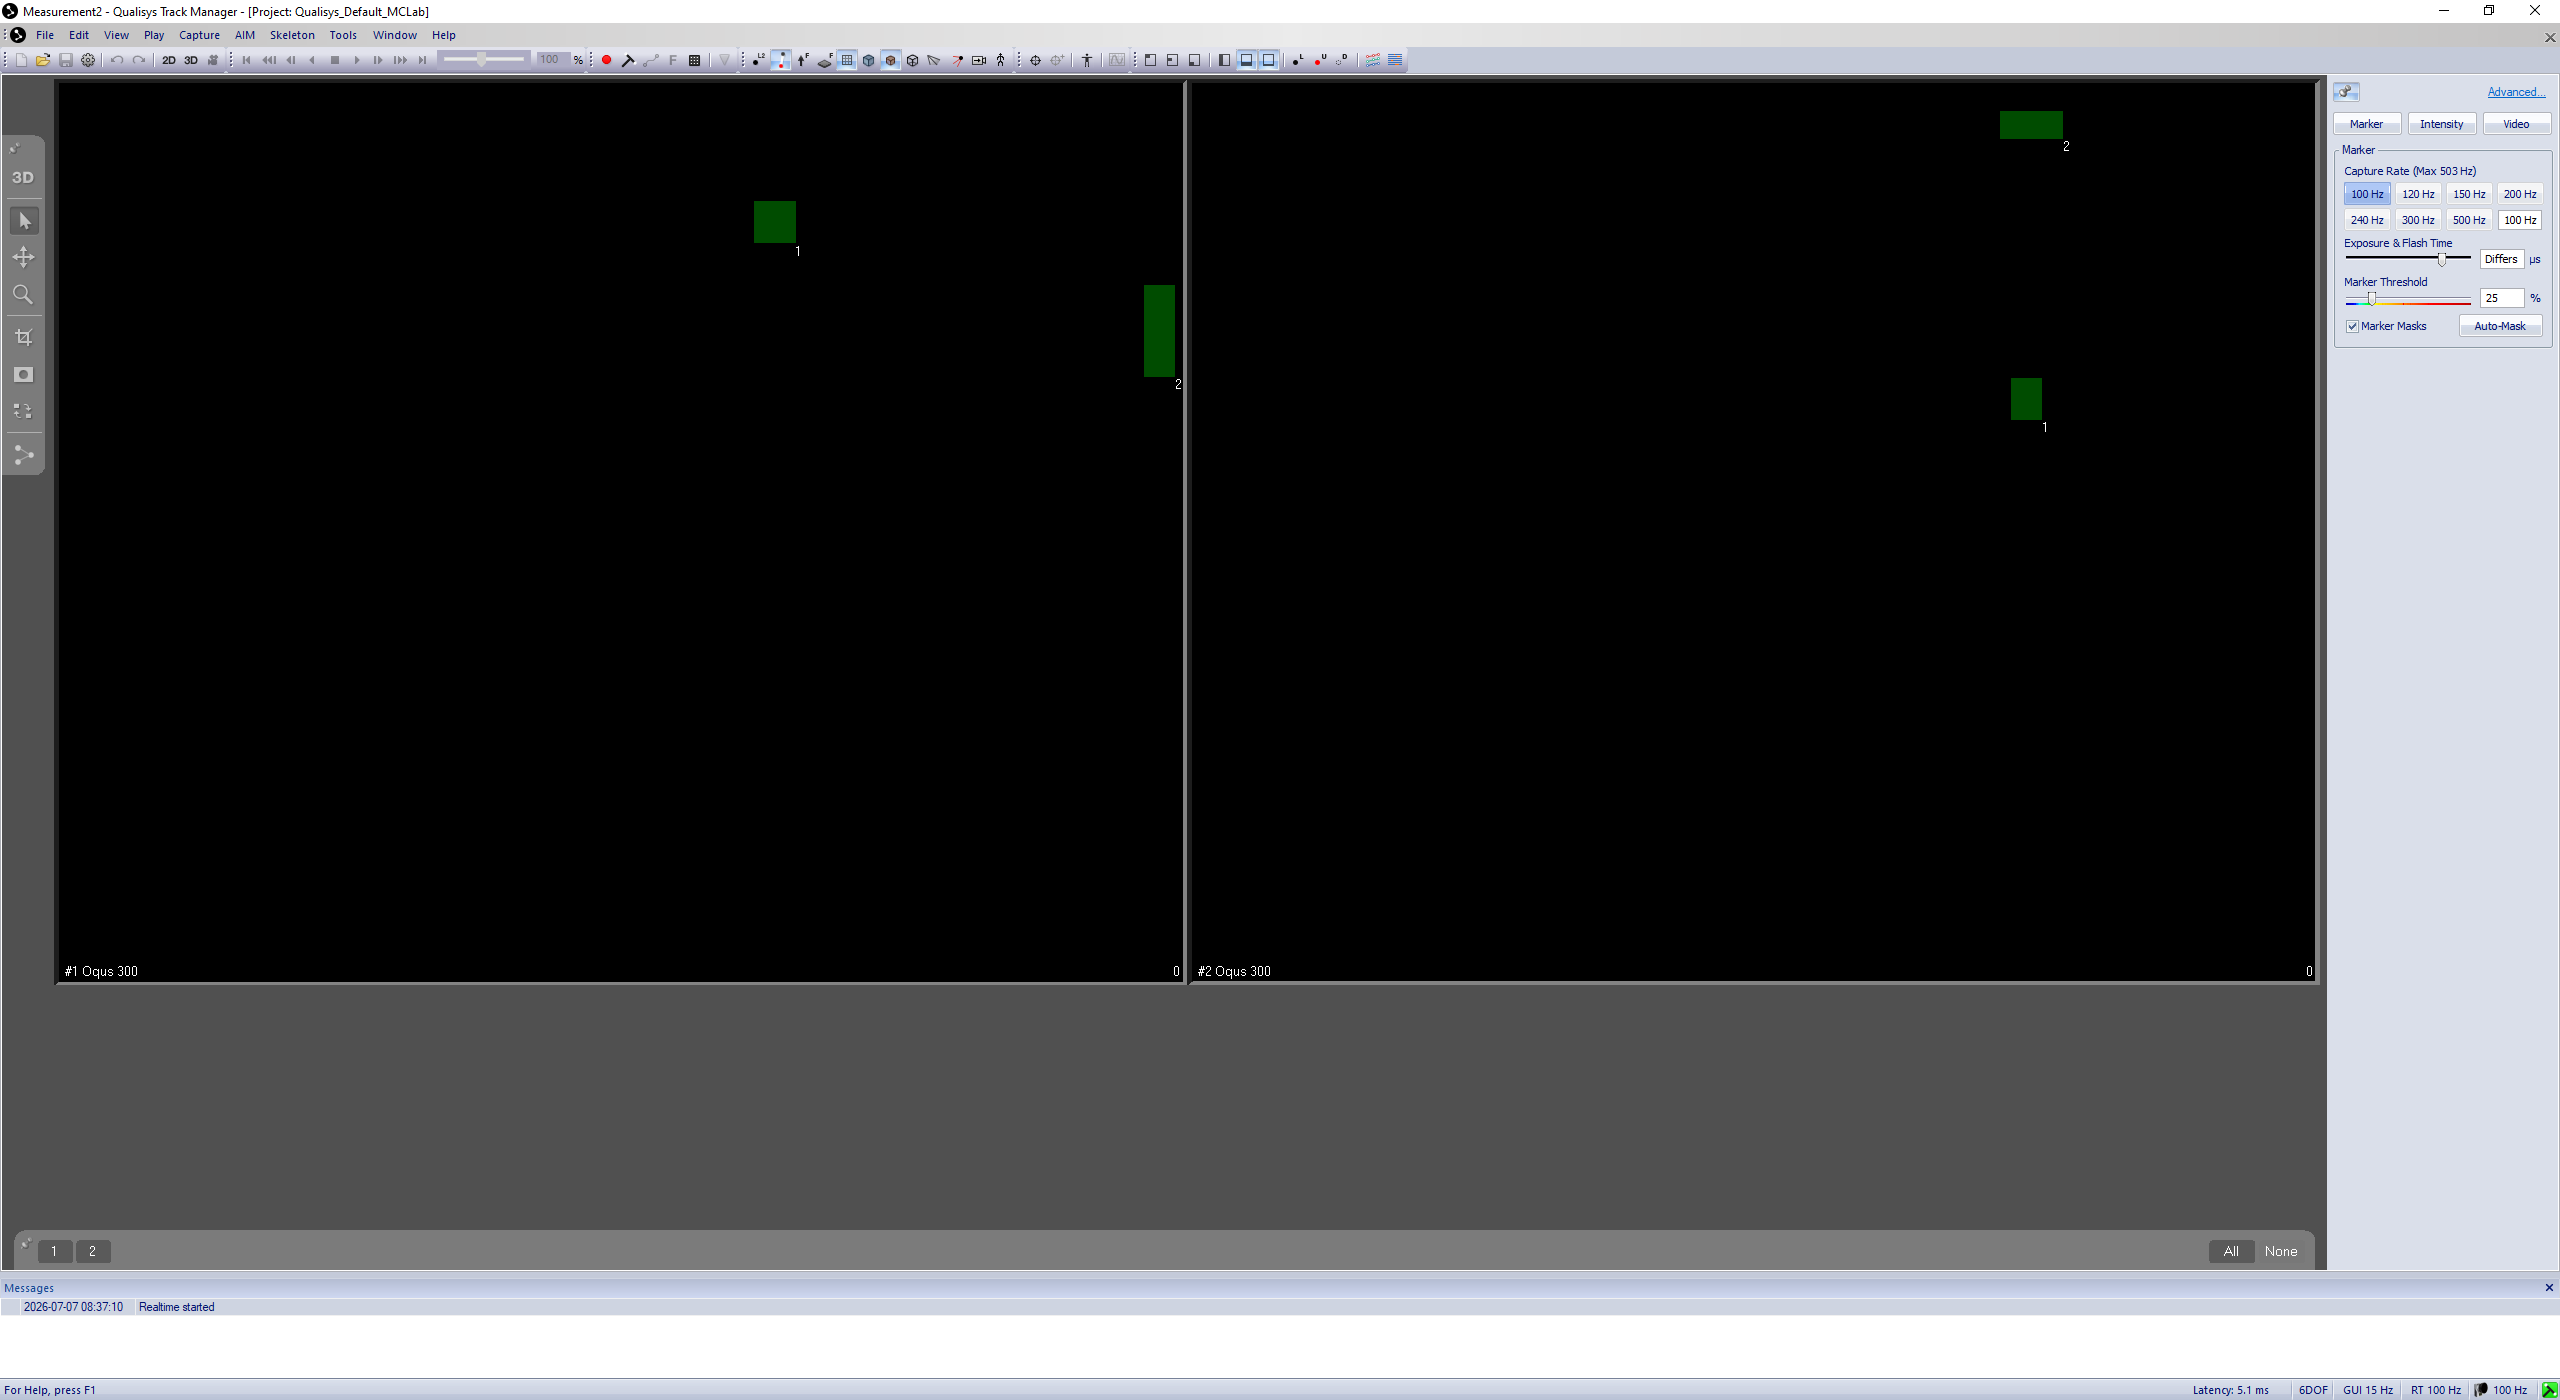
\includegraphics[width=0.5\textwidth]{QTM/3_2dview}
	\caption{Camera view in \textit{marker mode} click on the \textit{3D} icon on the left to enter \textit{3D mode}.}
	\label{fig:Cameraview}
\end{figure}

\begin{figure}[H]
	\centering
	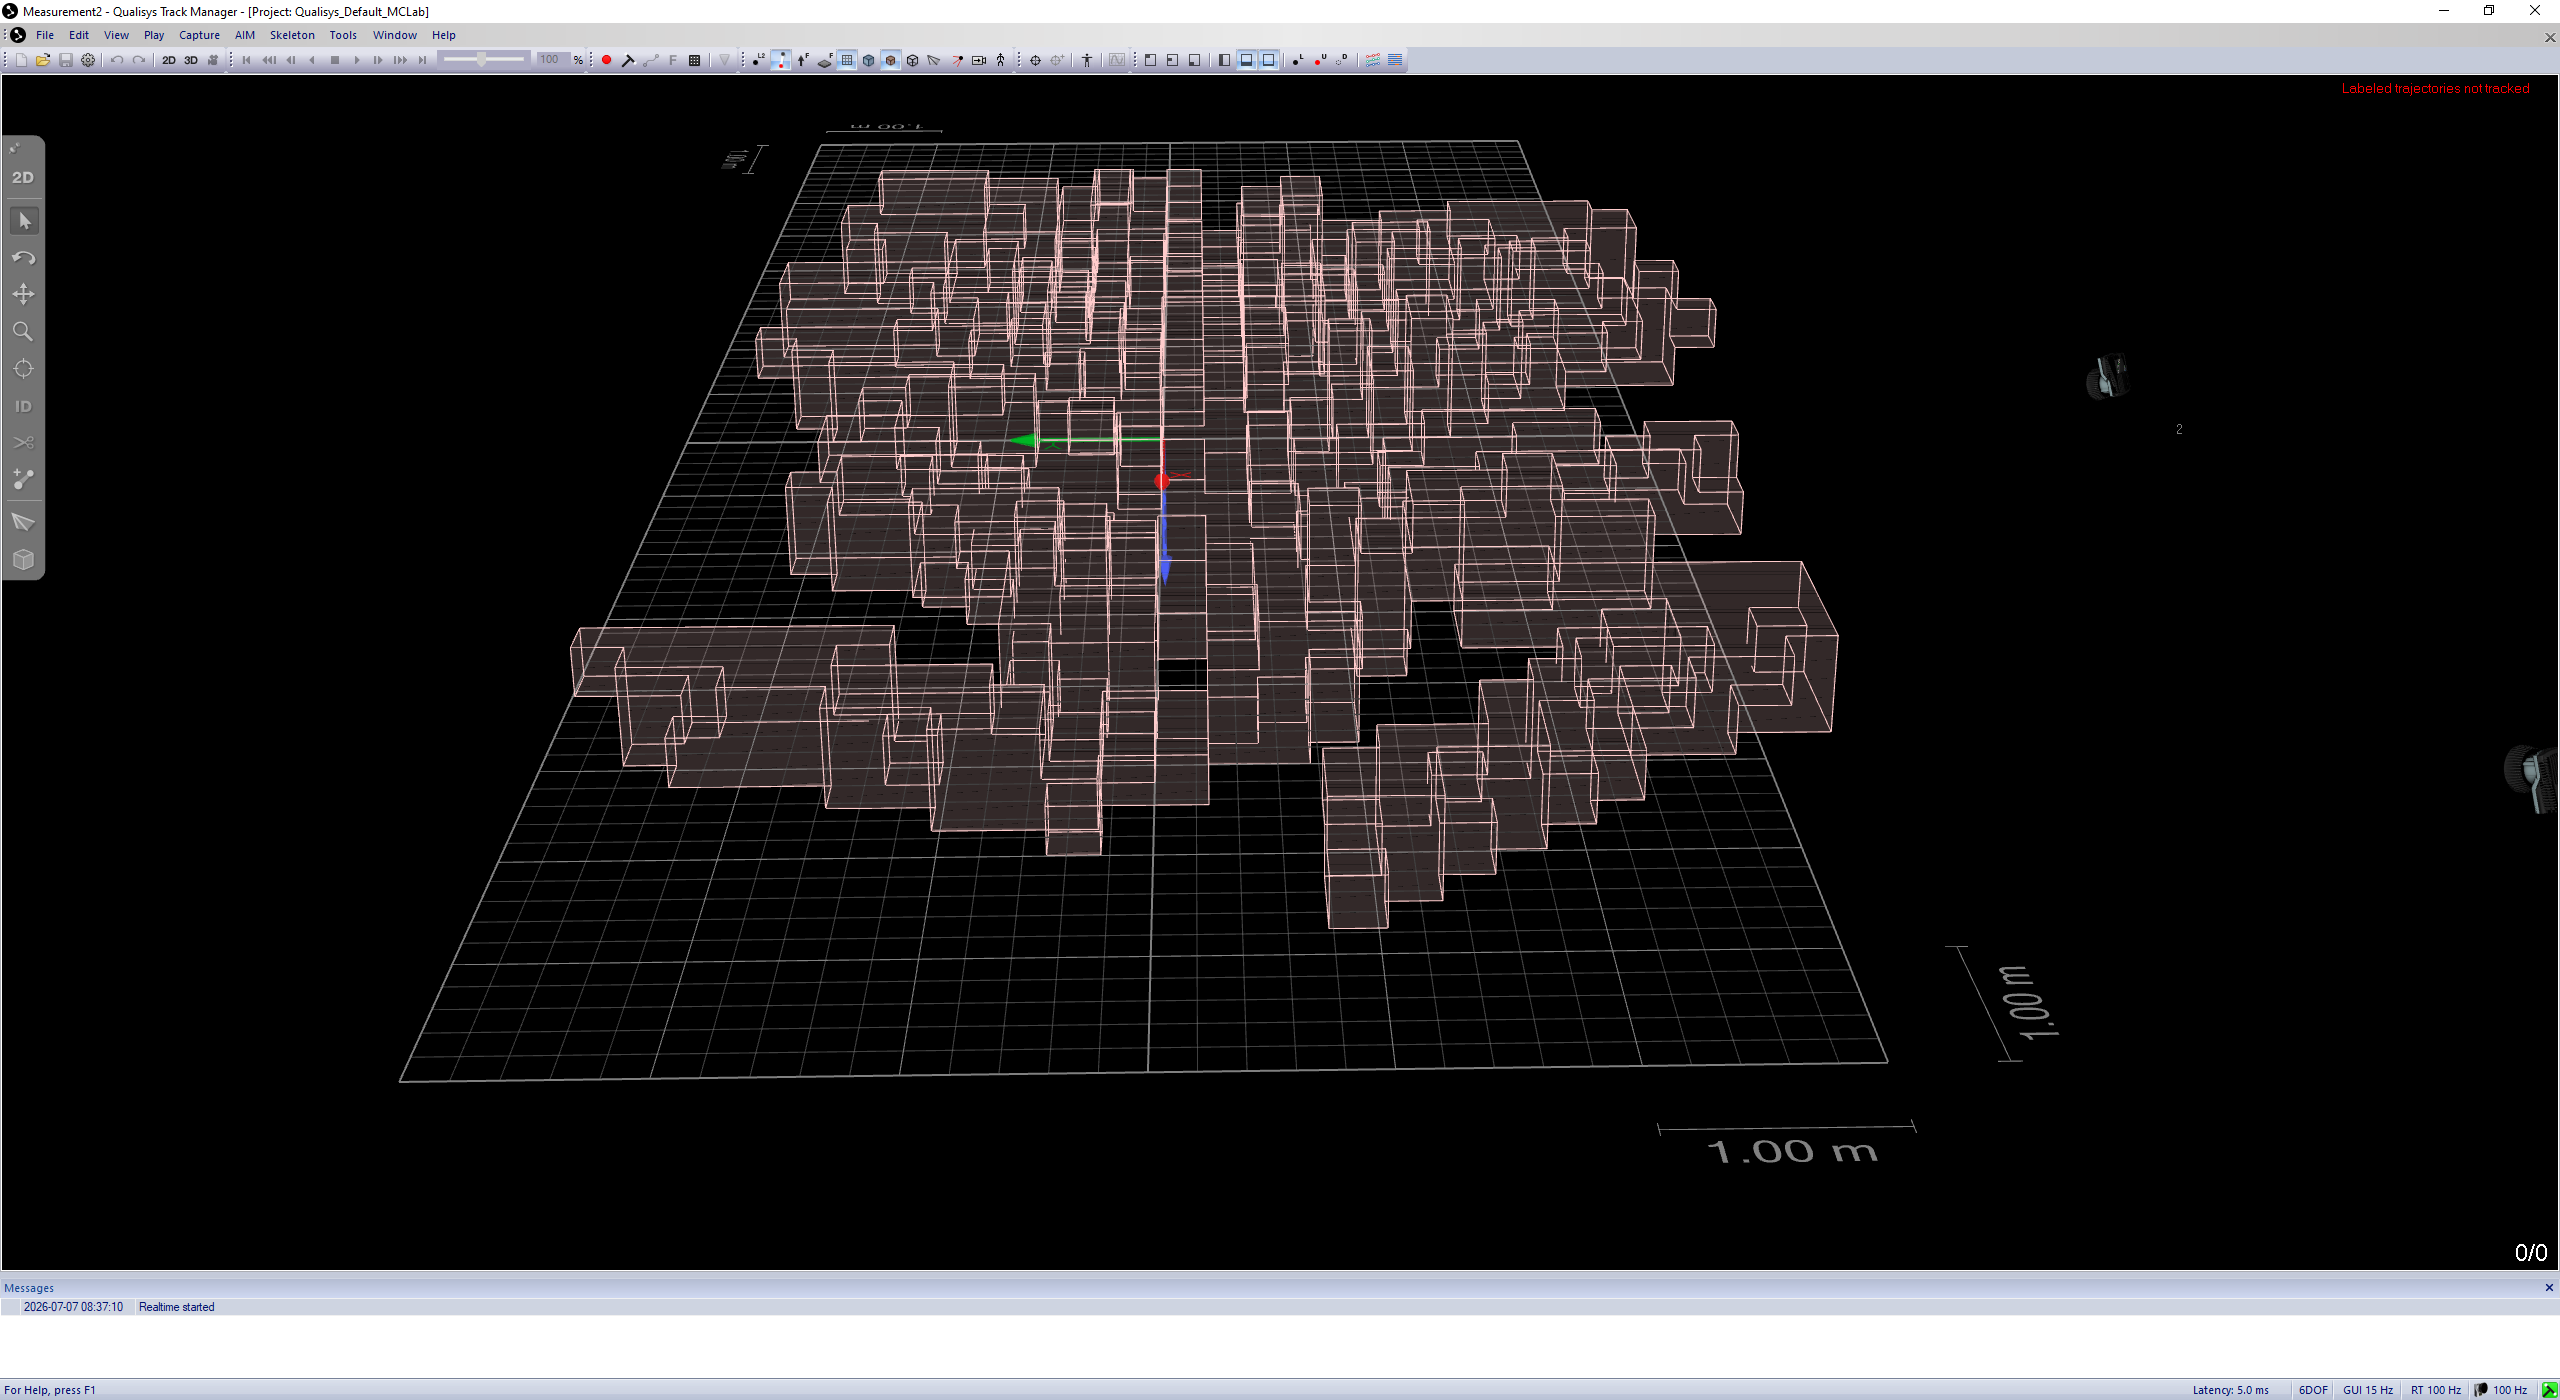
\includegraphics[width=0.5\textwidth]{QTM/4labframeofreferencewithcalibrated5volume}
	\caption{Lab frame of reference with the calibrated volume shown. Press \texttt{CTRL + D} or alternatively click \textit{view} on the top toolbar and then select \textit{Data Info 1} to show marker positions in \textit{2D}.}
	\label{fig:labFrame}
\end{figure}

\begin{figure}[H]
	\centering
	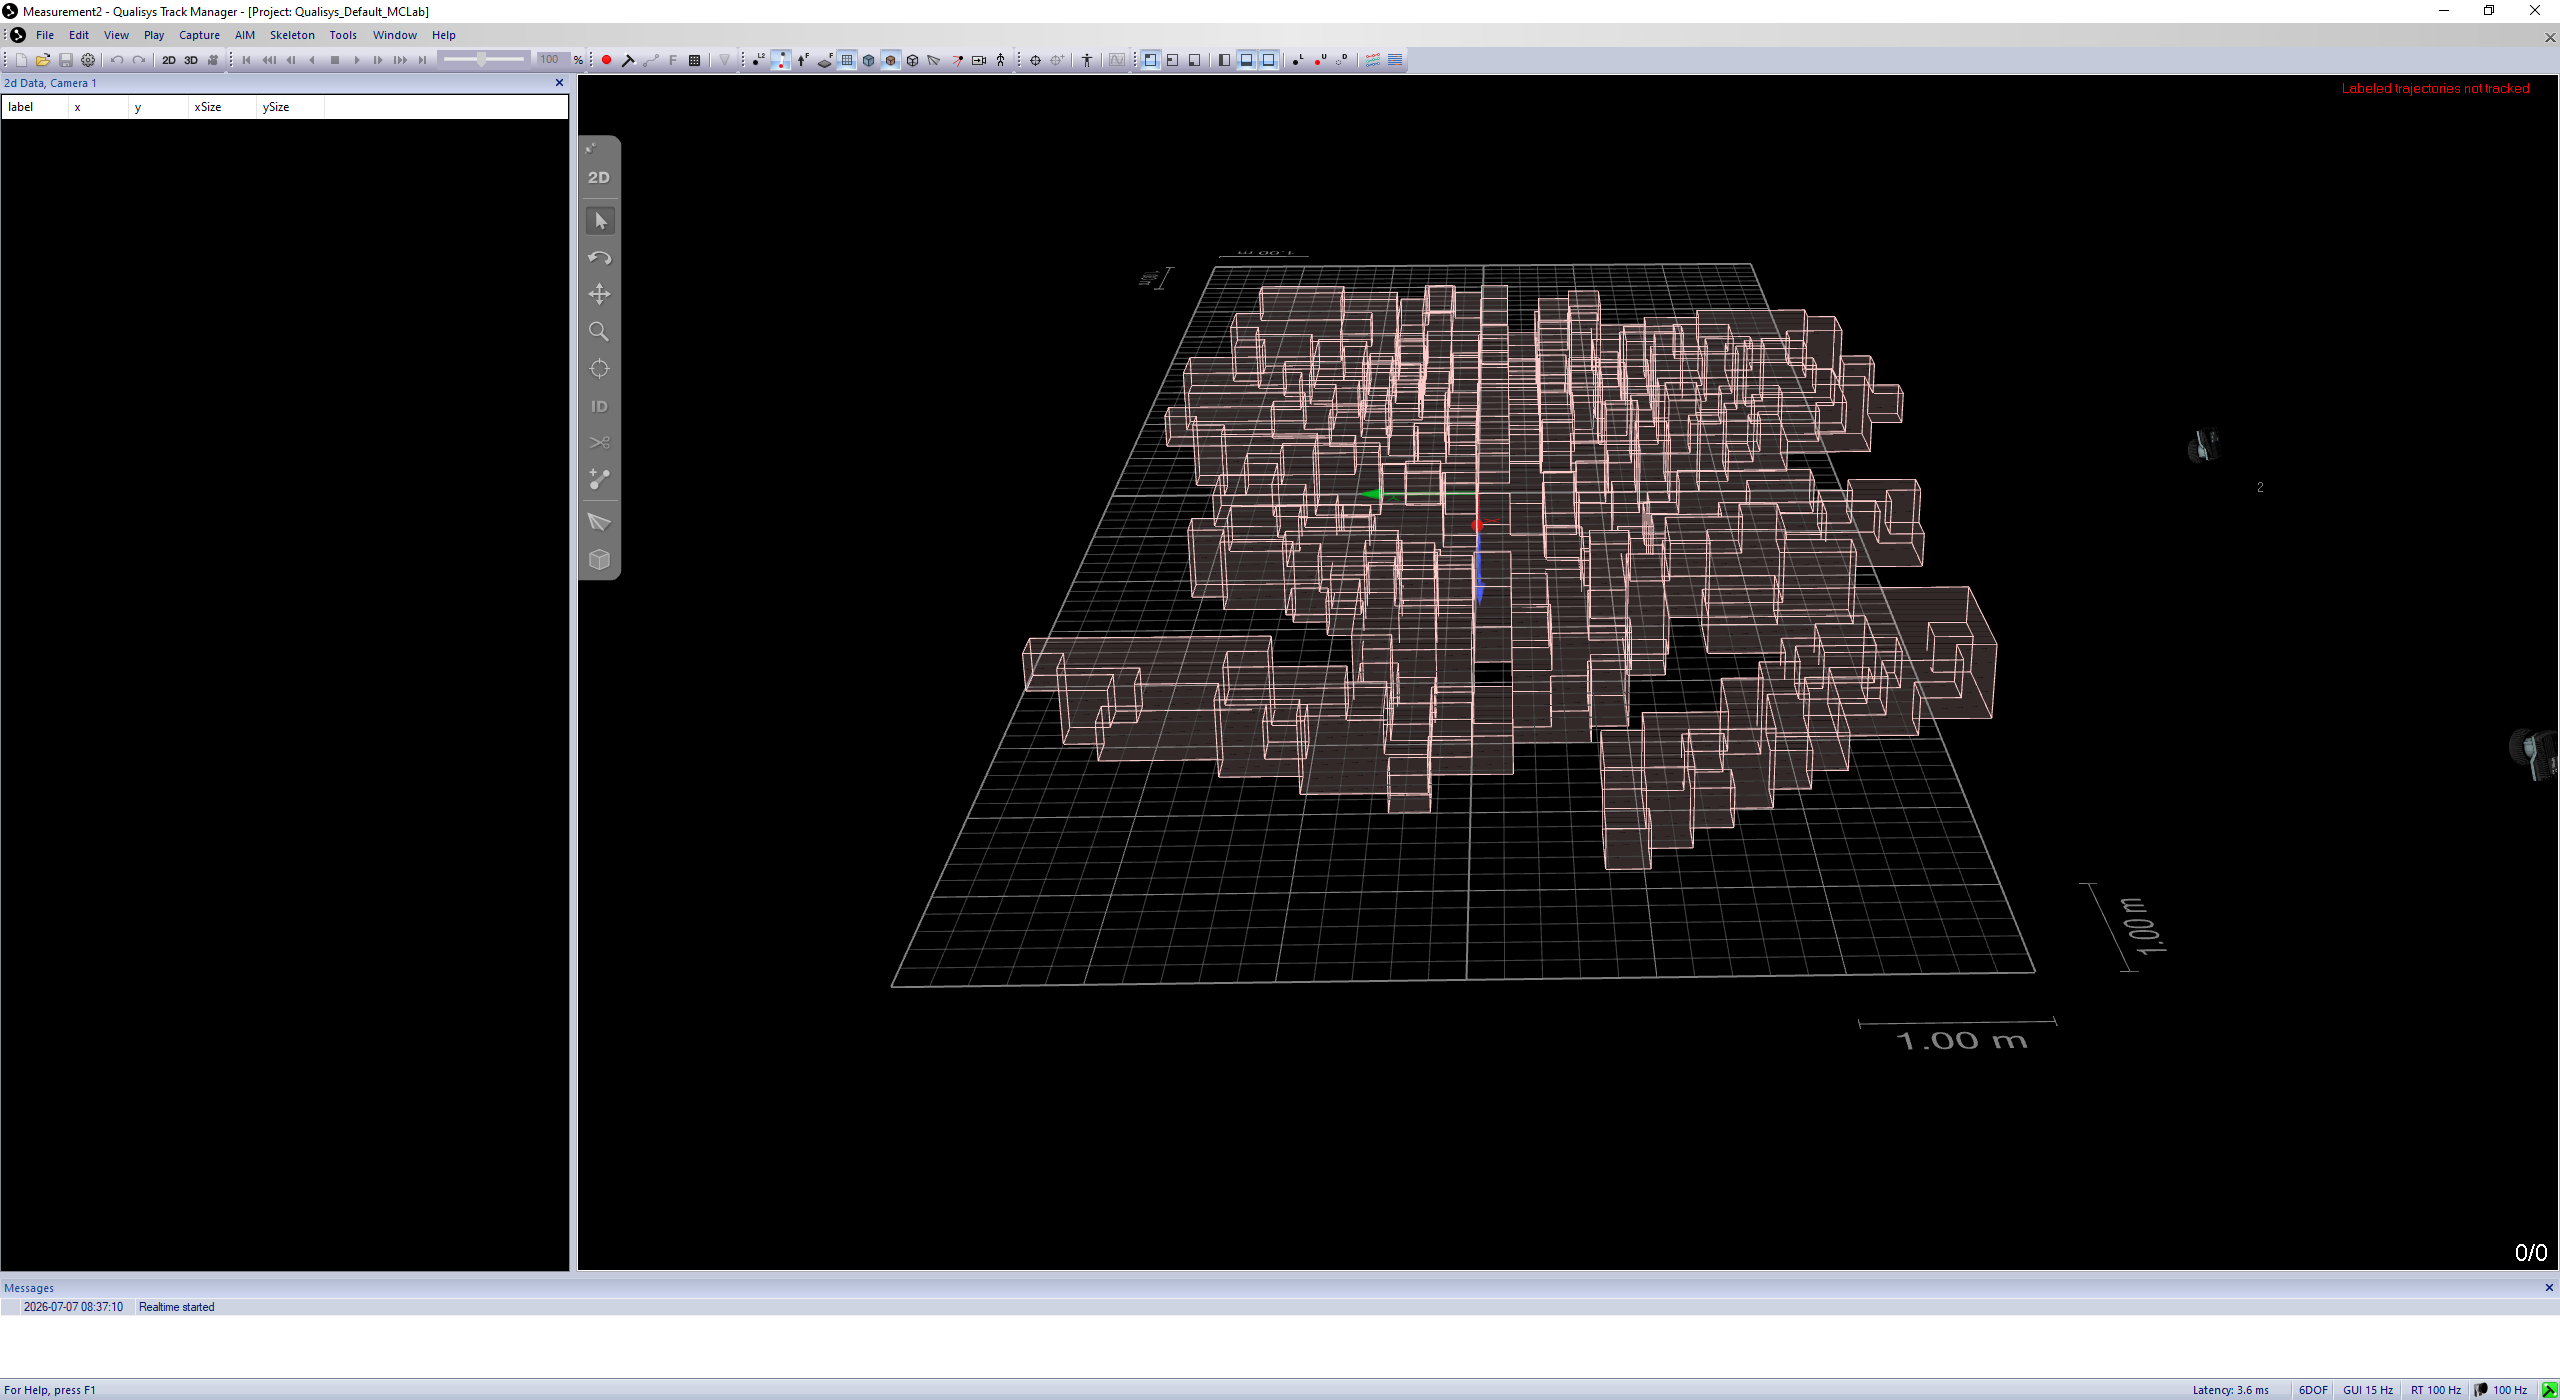
\includegraphics[width=0.5\textwidth]{QTM/5labframewith2dmarkercoordinates}
	\caption{Lab frame of reference with the calibrated volume and 2D marker position shown. Right click and select \textit{6DOF} to show rigid body coordinates.}
	\label{fig:3D}
\end{figure}

\begin{figure}[H]
	\centering
	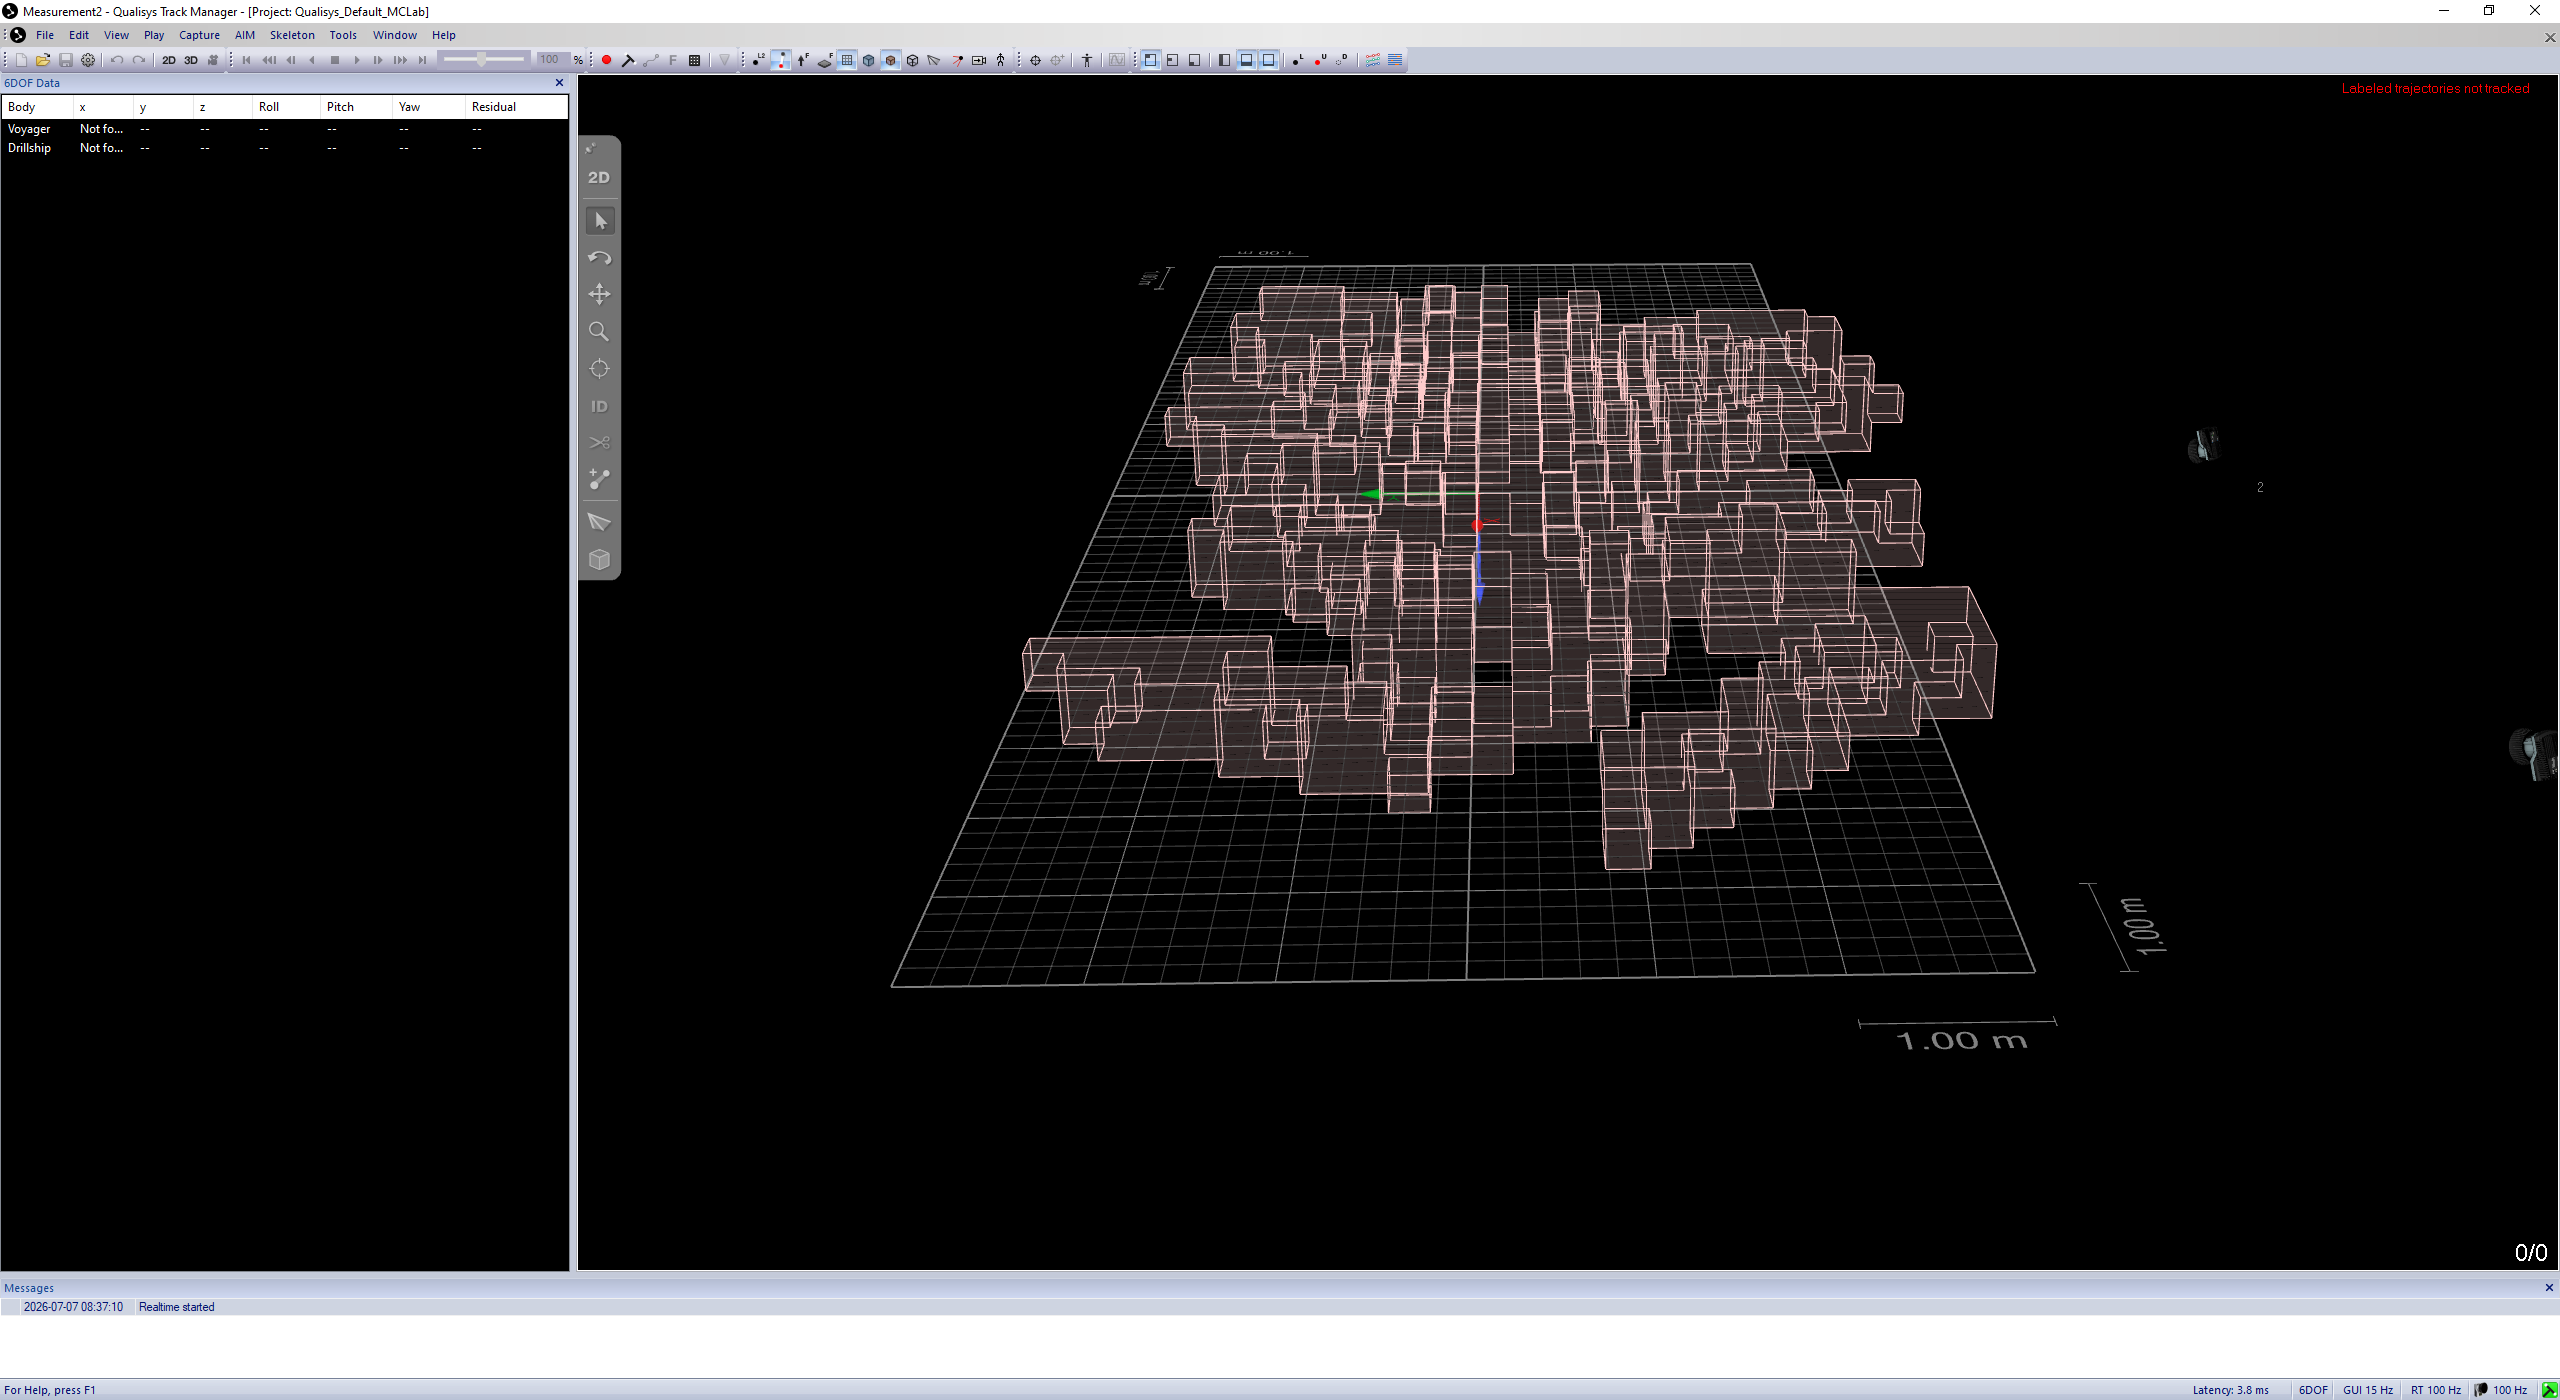
\includegraphics[width=0.5\textwidth]{QTM/Frame6dof}
	\caption{Lab frame of reference with the calibrated volume and rigid body coordinates.}
	\label{fig:6DOF}
\end{figure}

\begin{figure}[H]
	\centering
	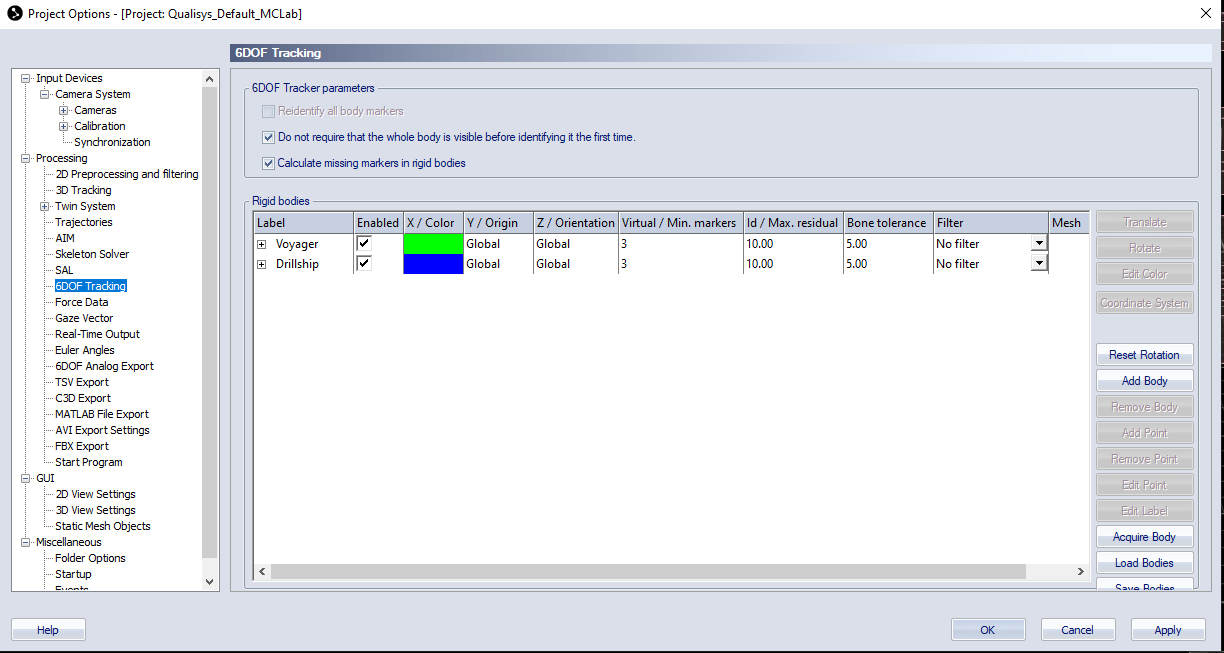
\includegraphics[width=0.5\textwidth]{QTM/7_6dofsettings}
	\caption{\textit{6DOF Settings} window were you can \textit{Add}, \textit{Acquire}, \textit{Load}, and \textit{Save} rigid bodies.}
	\label{fig:6DOFSettings}
\end{figure}


\begin{figure}[H]
	\centering
	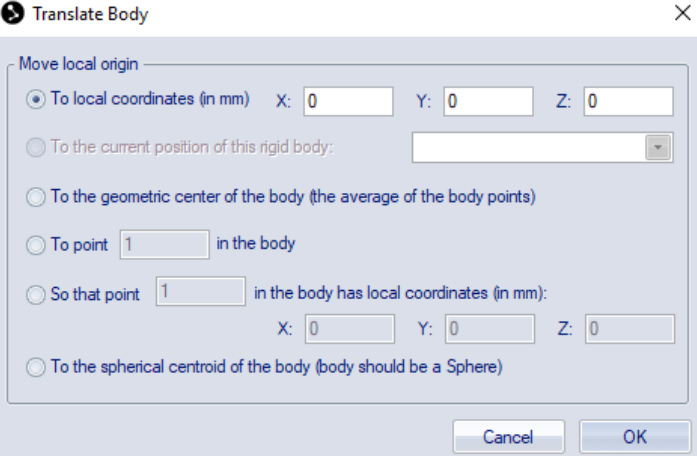
\includegraphics[width=0.5\textwidth]{QTM/8Translate}
	\caption{\emph{Translate Body} Settings where we can move the local origin.}
	\label{fig:6DOFSettings_translate}
\end{figure}

% Visual references for correct setup and common issues
\end{document}